\documentclass[12pt,a4paper]{article}
\usepackage{geometry}
\usepackage[numbers]{natbib}
\usepackage{amssymb, amsmath}
\usepackage{graphicx}
\usepackage{grffile}
\graphicspath{{../Figures/}}
\usepackage{gensymb}
\usepackage[font=small]{caption}
\usepackage[utf8]{inputenc}
\usepackage[english]{babel}
\usepackage{fancyhdr}
\usepackage[raggedright]{titlesec}
\usepackage{subcaption}
\usepackage{multirow}
\usepackage{dirtytalk}
\usepackage{framed}
\usepackage[normalem]{ulem}
\usepackage[pdftex,breaklinks]{hyperref}
\hypersetup{
  colorlinks   = true, %Colours links instead of ugly boxes
  urlcolor     = green, %Colour for external hyperlinks
  linkcolor    = blue, %Colour of internal links
  citecolor   = red %Colour of citations
}


\begin{document}
\author{Katrina Ashton}


\pagestyle{fancy}
\fancyhf{}
\rhead{\thepage}
\lhead{u5586882}

\section{What I've done}
\begin{itemize}
\item{Implemented the following in python using opencv:}
\begin{itemize}
\item Detecting SIFT features, and matching them (using brute force matcher)
\item Method 1. Calculating the essential matrix and using it to find R and t
\item Method 2. Getting a depth associated with feature points, and then aligning them using Kabsch algorithm, to find R and t
\item Graphing trajectories (component-wise) for both positions and quaternions
\end{itemize}
%\item{Added more to the appendices for the final report draft}
\end{itemize}

\section{Parts of report to look at}
\begin{itemize}
\item{Nothing new.}
\end{itemize}

\section{Questions}
\begin{itemize}
\item
\end{itemize}

\section{Comments}
\begin{itemize}
\item Pieter is using the new RealSense on the TX2, so it might be a bit tricky to run code for the R200 on it. 
\item The timestamps for the ground truth, rgb and depth images are not aligned, and there are not the same number of each. Right now I'm just reading in the rgb and depth images in order and matching them up that way, but I should actually associate a depth image to the rgb using the timestamps.
\item I should convert to axis-angle to compare the rotations rather than using the quaternions (although I'm not sure how to graph that).
\item The registered trajectories are very different to the ground truth. In particular, the ground truth has almost no variation in z but all components vary in the registered trajectories. I'm not sure if the issue is poor registration or issues converting between the various coordinates (does z in the ground truth correspond to y in the image? -- and x to z, y to x).
\item The position trajectories also have major scaling issues, and the registration with depth increases massively.
\item Need to quantify the differences, but will probably need to sort out the time stamp alignment first.
\item There are a few frames where the matching couldn't find enough good points (need at least 6) and so I skipped them. I also think my bound for good points might be a bit high. I might swap to a relative measure, as some frames have much better matches than others.
\end{itemize}

\begin{figure}[t!]
  \centering
  \begin{subfigure}[t]{0.3\textwidth}
  \centering
    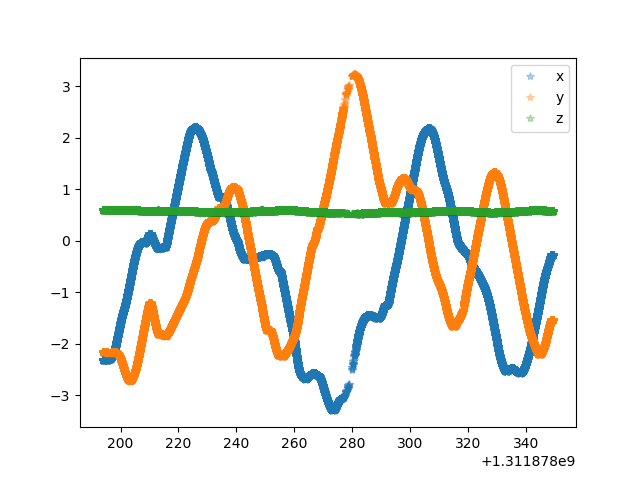
\includegraphics[width=45mm]{reg_graphs/180_no-rot-d/trj_gt.PNG}
  \caption{Position trajectory - ground truth}
  \end{subfigure} %
  ~
  \begin{subfigure}[t]{0.3\textwidth}
  \centering
    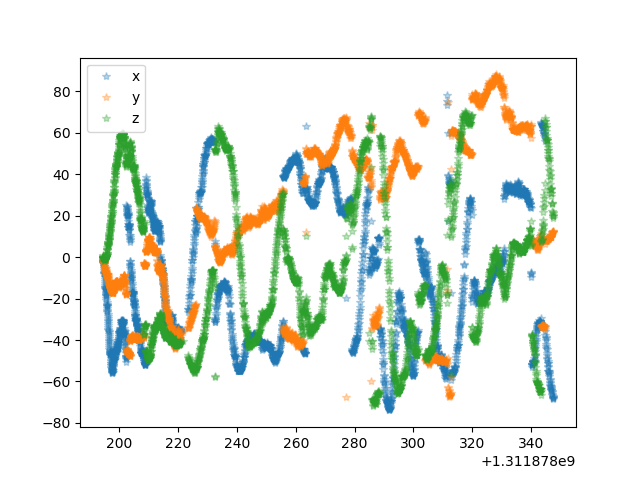
\includegraphics[width=45mm]{reg_graphs/180_no-rot-d/trj_rgb.PNG}
  \caption{Position trajectory - RGB only registration}
  \end{subfigure}%
  ~
  \begin{subfigure}[t]{0.3\textwidth}
  \centering
    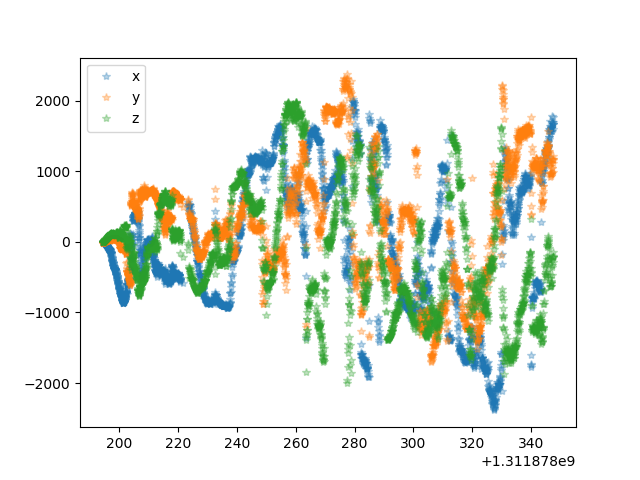
\includegraphics[width=45mm]{reg_graphs/180_no-rot-d/trj_d.PNG}
  \caption{Position trajectory - registration using depth}
  \end{subfigure}
  \caption{Comparison of position trajectories.}
\end{figure}

\begin{figure}[t!]
  \centering
  \begin{subfigure}[t]{0.3\textwidth}
  \centering
    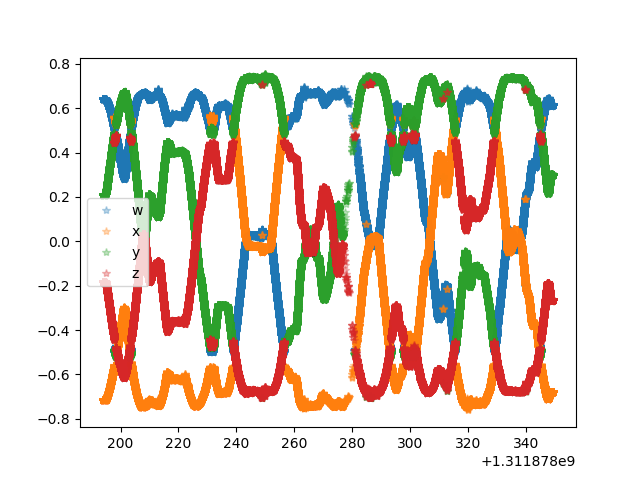
\includegraphics[width=45mm]{reg_graphs/180_no-rot-d/qtrj_gt.PNG}
  \caption{Quaternion trajectory - ground truth}
  \end{subfigure} %
  ~
  \begin{subfigure}[t]{0.3\textwidth}
  \centering
    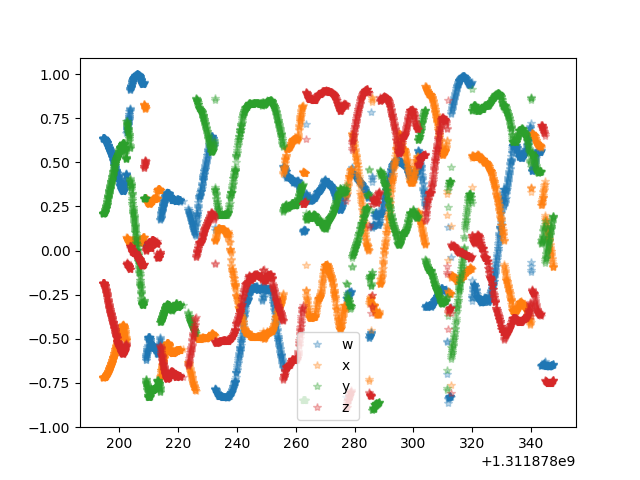
\includegraphics[width=45mm]{reg_graphs/180_no-rot-d/qtrj_rgb.PNG}
  \caption{Quaternion trajectory - RGB only registration}
  \end{subfigure}%
  ~
  \begin{subfigure}[t]{0.3\textwidth}
  \centering
    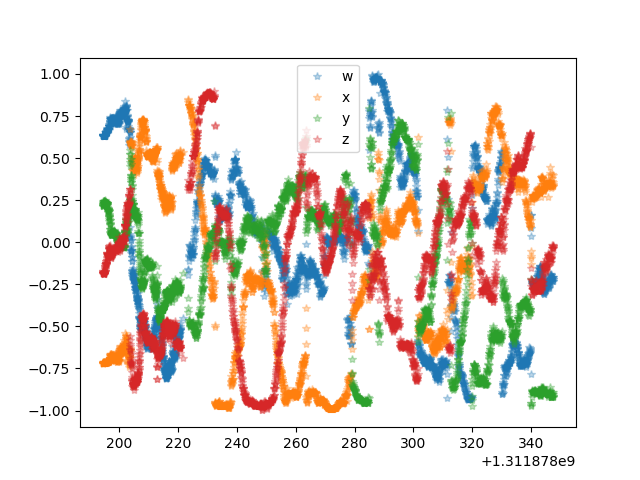
\includegraphics[width=45mm]{reg_graphs/180_no-rot-d/qtrj_d.PNG}
  \caption{Quaternion trajectory - registration using depth}
  \end{subfigure}
  \caption{Comparison of quaternion trajectories.}
\end{figure}


\section{Stuff to do}
\begin{itemize}
\item \sout{Fix quadcopter}
\item Adjust quadcopter trajectory so that it can see the top box
\item Investigate data
\begin{itemize}
\item \sout{Investigate boxes to determine which ones can be picked up as point clouds}
\item \sout{Investigate RealSense cameras, compare the two cameras and using them on TX1/TX2 or Windows/Ubuntu}
\end{itemize}
\item Investigate registration algorithm
\begin{itemize}
\item Generate 3D object in MATLAB that I can get points from from various camera poses (may also need to get RGB and depth images if we're going with that approach?)
\item Apply registration algorithm to generated point clouds (ground truth known) -- without noise first, then add noise. Get error in true and estimated translation and rotation.
\end{itemize}
\item Reading
\begin{itemize}
\item \sout{Incorporating RGB and depth images -- feature matching (papers you sent me)}
\item Write up summary of main points (parts of the algorithm, choices with advantages/disadvantages)
\item See if more recent papers have made advancements
\end{itemize}
\end{itemize}

\end{document}